\documentclass[11pt,a4paper]{article}

\usepackage[T1]{fontenc}
\usepackage[utf8]{inputenc}
\usepackage{lmodern}
\usepackage[margin=2.5cm]{geometry}
\usepackage{microtype}
\usepackage{graphicx}
\usepackage{booktabs}
\usepackage{array}
\usepackage{ragged2e}
\usepackage{enumitem}
\usepackage{amsmath}
\usepackage{xurl}
\def\UrlBreaks{\do\/\do\-\do\_}
\usepackage[hidelinks]{hyperref}
\usepackage{caption}
\usepackage{float}
\captionsetup{font=small,labelfont=bf,justification=raggedright,singlelinecheck=false}

\graphicspath{{figures/}{../../tasks/task02-ttp/diagrams/}}

\setlength{\parskip}{0.35em}
\setlength{\parindent}{0pt}
\setlength{\emergencystretch}{2em}
\renewcommand{\arraystretch}{1.15}

\title{\textbf{APT29 and the SolarWinds Supply-Chain Compromise}\\[0.4em]
\large From SUNSPOT to a Controlled Recreation in Mininet and Docker}

\author{CDCI Assignment 1}
\date{November 2026}

\begin{document}

\maketitle

\begin{abstract}
\noindent
This article examines APT29's compromise of the SolarWinds Orion build pipeline and a controlled recreation of its delivery and command-and-control stages. It traces the actor's history, the techniques used in the incident, the public evidence of its infrastructure and victims, and the countermeasures proposed for each stage. The recreation uses Mininet and Docker to publish a signed package that carries a component, then reproduces the DNS check-in, mode selection and operator tasking, using a fixed handoff name that must return a CNAME before any tasking. The client accepts a malicious package that the supplier pipeline signed, which isolates the signing step from any build compromise. The article states where the lab diverges from the incident, reviews six peer-reviewed papers on supply-chain integrity and DNS detection, and derives a research question on combining provenance checks with DNS monitoring. It does not claim to reproduce SUNBURST or to measure the effectiveness of the countermeasures it discusses.
\end{abstract}

{\raggedright\hyphenpenalty=10000\exhyphenpenalty=10000\noindent\textbf{Keywords:} APT29; SolarWinds; SUNBURST; software supply chain; Mininet; DNS monitoring; reproducible builds.\par}

\vspace{1em}

\section{Introduction}

In December 2020, FireEye disclosed that a backdoor had been distributed to customers of SolarWinds inside a correctly signed update of the Orion IT-monitoring platform. The campaign was attributed to the SVR by U.S. and UK authorities, and MITRE tracks the activity as APT29~\cite{mitre-apt29,aa22-110a}. The incident matters beyond its victim list because nothing in the delivery path was broken. The supplier's build system produced the malicious component, the supplier's signing process signed it, and customers installed it through the update channel they had been told to trust.

The incident is reconstructed from public reporting, with each event tied to the source that reported it. The recreation in Section~\ref{sec:recreation} follows the behaviour Mandiant and CrowdStrike documented; it does not run the actor's binaries~\cite{mandiant-sunburst-details,crowdstrike-sunspot}.

The report covers the group's history, the techniques and infrastructure behind the incident, the victims and their losses, and a lab that reproduces the trust failure rather than the malware. It closes with six peer-reviewed papers and a research question. A valid signature answers whether the supplier signed an artefact. It does not answer whether the build that produced the artefact was clean.

\section{The actor}
\label{sec:actor}

APT29 is tracked under several names. Microsoft calls the group Midnight Blizzard or NOBELIUM, Mandiant used UNC2452 for the SolarWinds activity before merging it into APT29~\cite{mandiant-unc2452}, and older reporting uses Cozy Bear or The Dukes~\cite{mitre-apt29,eset-ghost}. A 2022 joint advisory from agencies in the United States, Australia, Canada, New Zealand, and the United Kingdom states that the SVR has run cyber operations since at least 2008 and lists APT29 among the names used for those actors~\cite{aa22-110a}.

ESET reported that Operation Ghost began in 2013 and was still active in 2019, targeting foreign ministries in at least three European countries and an EU member state's embassy in Washington~\cite{eset-ghost}. In the Democratic National Committee breach, CrowdStrike found Cozy Bear on the network from summer 2015 and a separate actor, Fancy Bear, from April 2016, with no evidence that the two worked together~\cite{crowdstrike-dnc}. In July 2020, the UK National Cyber Security Centre and Canada's Communications Security Establishment reported that APT29 had targeted organisations involved in COVID-19 vaccine development in Canada, the United States, and the United Kingdom, with the likely aim of obtaining vaccine research~\cite{ncsc-vaccine}.

After SolarWinds the group changed access methods without changing its target set. It exploited JetBrains TeamCity in 2023~\cite{aa23-347a}, then ran phishing campaigns against German political parties, European diplomats, and more than 100 organisations in 2024 and 2025~\cite{mandiant-wineloader,ms-rdp,checkpoint-2025}. Check Point called the 2025 attribution likely, citing overlap with earlier activity and similar code.

\section{The SolarWinds operation}
\label{sec:operation}

\begin{figure}[t]
\centering
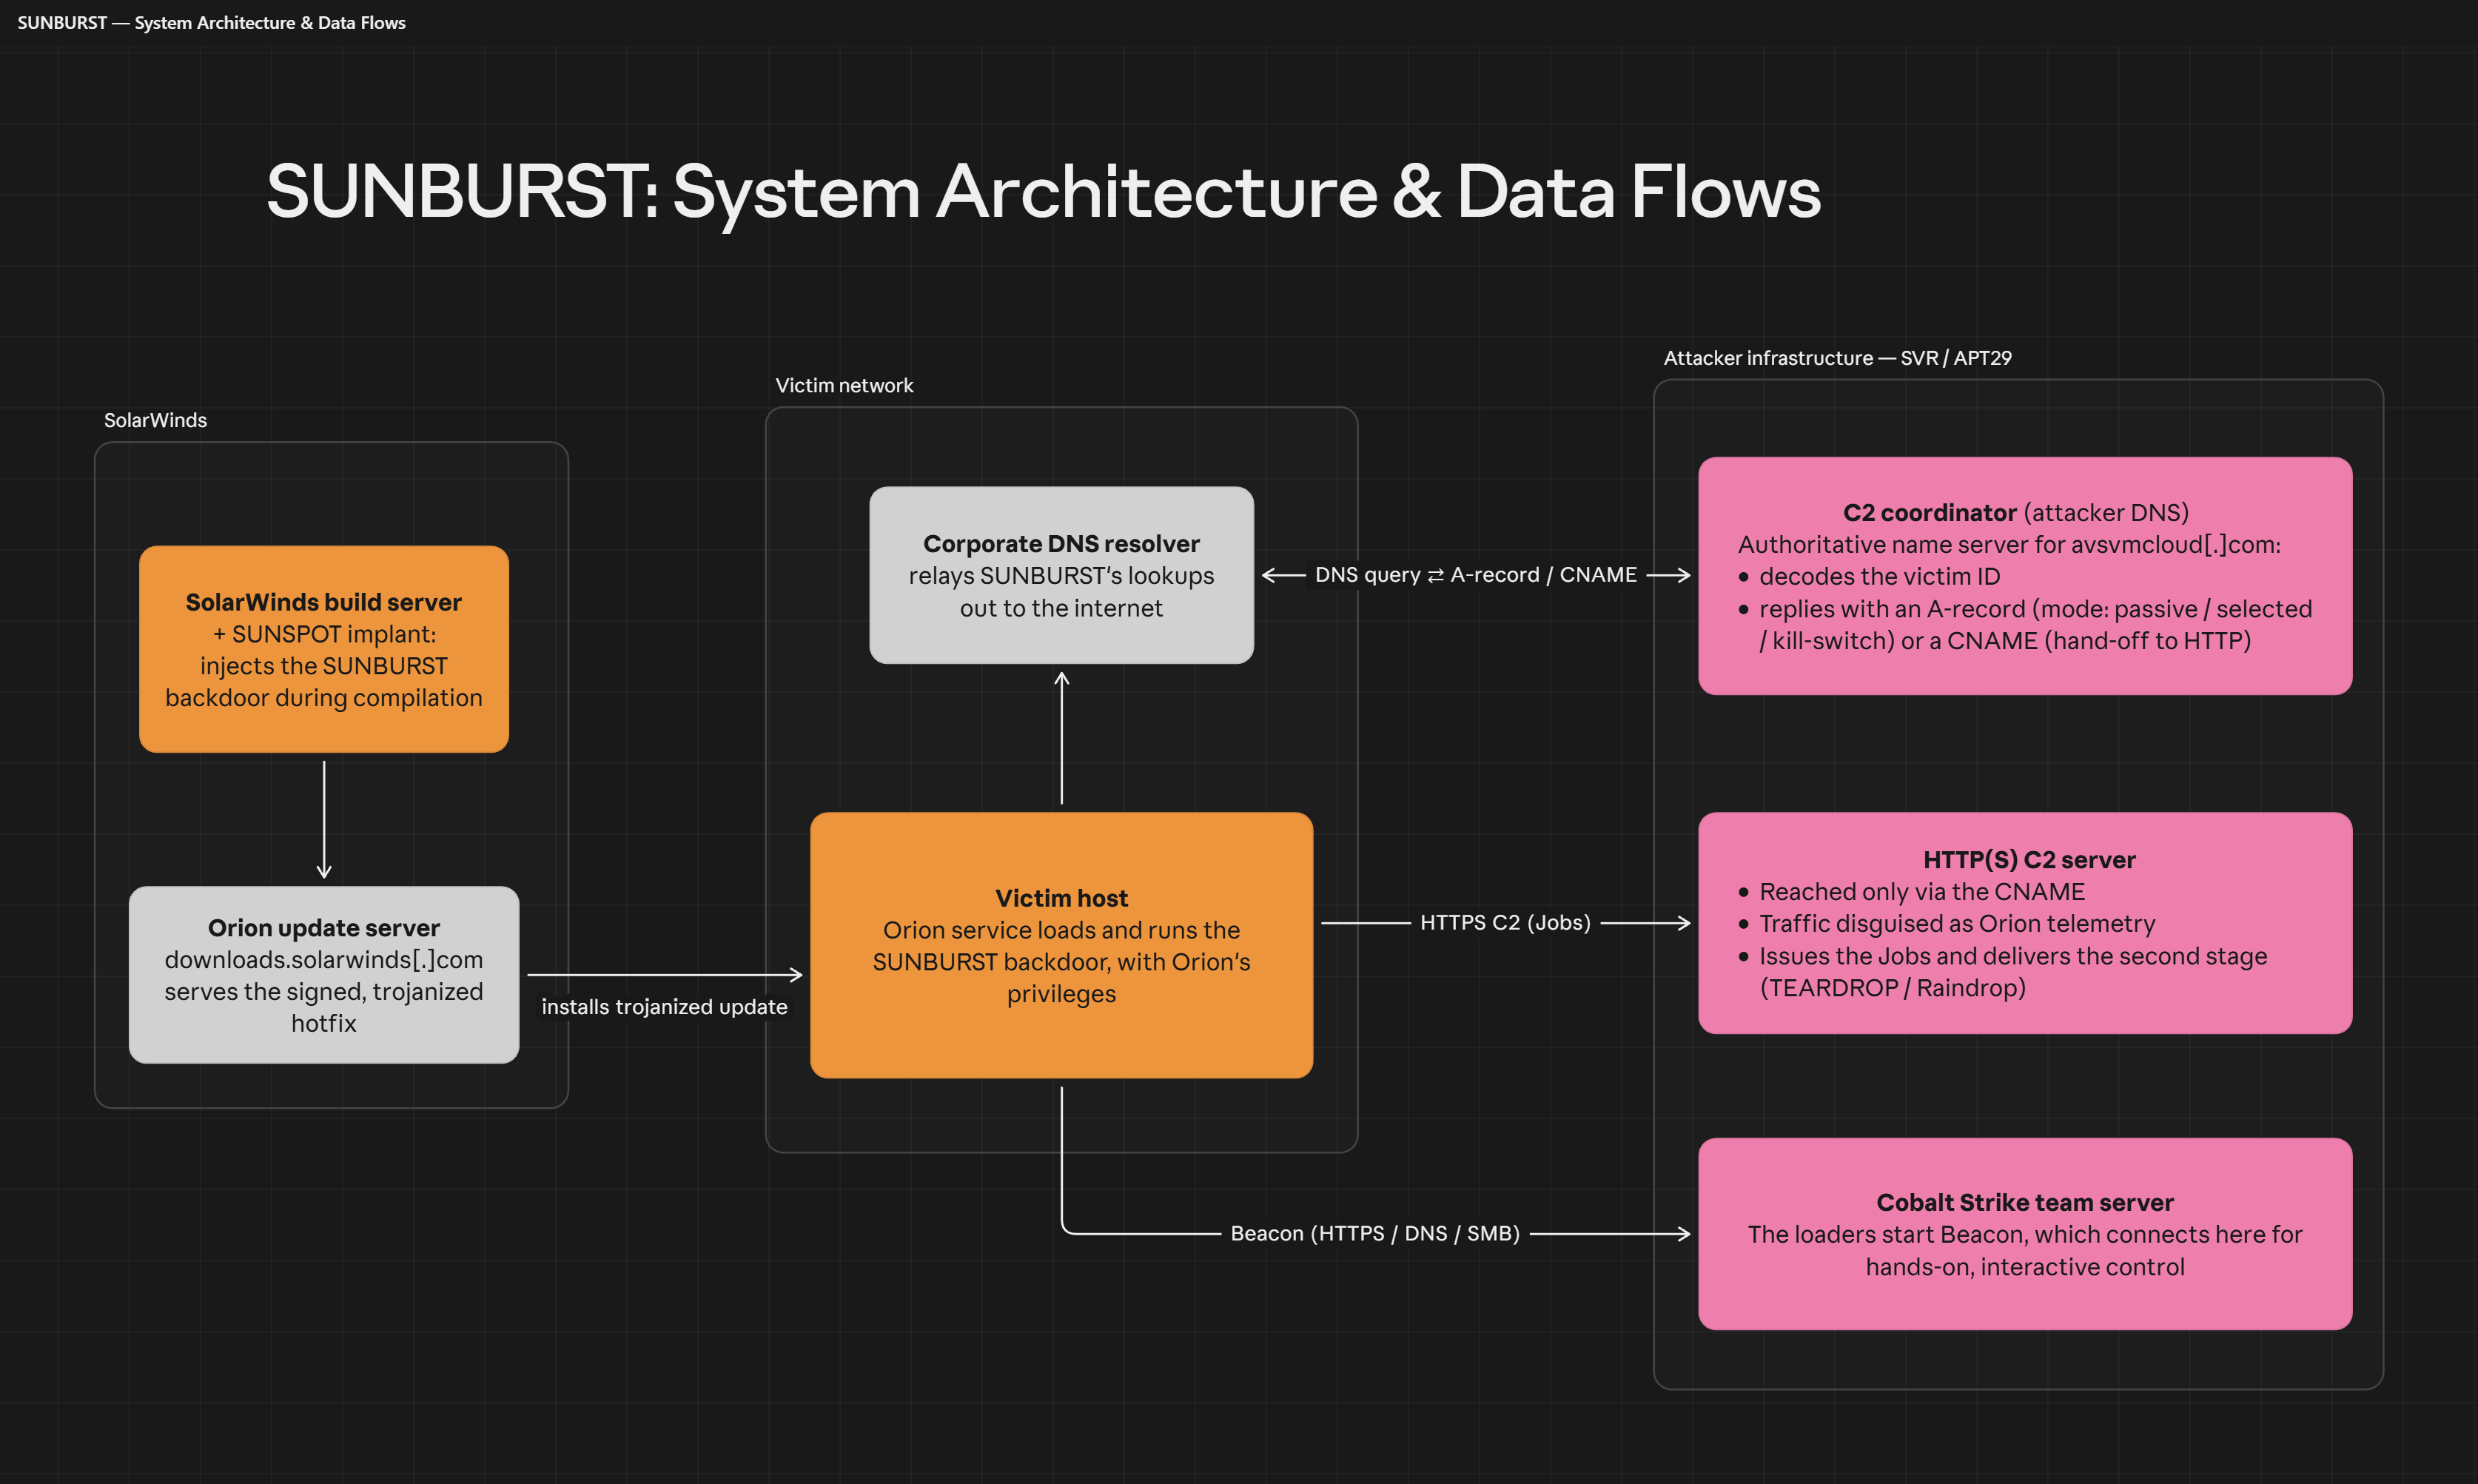
\includegraphics[width=0.92\textwidth,keepaspectratio]{architecture.png}
\caption{Attack architecture for the SolarWinds compromise, as documented in the Task~2 analysis. The build compromise precedes distribution; the lab in Section~\ref{sec:recreation} models the right-hand side of this path.}
\label{fig:architecture}
\end{figure}

Figure~\ref{fig:architecture} places the build compromise at the start of the chain: the actor works inside the supplier's environment, and every later stage inherits the supplier's legitimacy. The subsections below follow that path.

\subsection{Build compromise}

SolarWinds stated that it could not determine how the attackers first entered its network~\cite{solarwinds-sec}. CrowdStrike analysed an implant called SUNSPOT that ran on the Orion build server as \texttt{taskhostsvc.exe}, kept alive by a scheduled task. It waited for \texttt{MsBuild.exe}, read the build command line from process memory, and compared the MD5 of both the original source file and the backdoored copy against hardcoded values before replacing \texttt{InventoryManager.cs}. The original was kept as a \texttt{.bk} file and restored when the build exited, so the source repository looked untouched, and the edits were wrapped in \texttt{\#pragma warning disable}~\cite{crowdstrike-sunspot}.

The result was an Orion component containing SUNBURST. SolarWinds signed it through its normal release process and published it as a routine update~\cite{mandiant-campaign,mandiant-sunburst-details}.

\subsection{Dormancy and check-in}

SUNBURST did not act immediately. It required an Active Directory domain, stopped if the domain resembled a SolarWinds test environment, compared running processes against a list of analysis tools, and waited until the plugin file was 12 to 14 days old~\cite{mandiant-sunburst-details}. It then built a subdomain under \texttt{avsvmcloud[.]com} with a domain generation algorithm, encoding a user identifier and the victim's domain, and resolved it with the system DNS client~\cite{mandiant-sunburst-details}.

The coordinator answered with an A record, and the address range set the next state. Truncate (3) disabled the implant. New (4) kept it passive and checking in. Append (5) made it active. A CNAME response supplied the host for HTTPS command and control, which the malware required because it could not use a raw address~\cite{mandiant-sunburst-details}.

\subsection{Command and control and follow-on}

Active traffic imitated the Orion Improvement Program (OIP): JSON documents shaped like product telemetry, with fields such as \texttt{userId}, \texttt{sessionID}, and a \texttt{steps} array, and commands hidden in the response body. Payloads up to 10,000 bytes were wrapped as JSON; larger messages were sent unmodified. The tasking covered process execution, file transfer, registry access, and reboot~\cite{mandiant-sunburst-details}. On selected victims, operators delivered second-stage loaders. TEARDROP ran in memory, opened a file named \texttt{gracious\_truth.jpg}, and in at least one case used an Image File Execution Options value on \texttt{dllhost.exe} to start Cobalt Strike Beacon~\cite{microsoft-teardrop}. Raindrop was a second loader that served the same purpose~\cite{microsoft-teardrop}. Operators then used AdFind for directory enumeration and stole credentials including through DCSync~\cite{mandiant-campaign}. To reach Microsoft 365 mail, they compromised a SAML signing certificate and created valid tokens for accounts they did not control~\cite{cisa-aa20-352a}.

Exposure and compromise were different figures. Up to about 18,000 customers downloaded the affected builds, SolarWinds estimated that fewer than 100 were compromised, and nine U.S. federal agencies were among them~\cite{gao}.

\section{Techniques, indicators and vulnerabilities}
\label{sec:techniques}

Delivering and installing the backdoor exploited no software vulnerability, and both steps used the supplier's own build, signing and distribution processes. Later credential and cloud steps did not. That absence matters analytically: a vulnerability-management programme would not have seen this chain, because there was no vulnerable service to patch.

Table~\ref{tab:attack} lists the ATT\&CK techniques that carry the incident. Table~\ref{tab:iocs} lists the indicators published by Microsoft, CrowdStrike, and CISA. Table~\ref{tab:cves} lists vulnerabilities the group used in other campaigns for initial access; none belongs to the Orion compromise~\cite{nsa-svr}.

\begin{table}[H]
\centering
\footnotesize
\hyphenpenalty=10000
\caption{Core ATT\&CK techniques in the SolarWinds chain. IDs follow Enterprise v20.1.}
\label{tab:attack}
\begin{tabular}{@{}>{\RaggedRight}p{1.8cm}>{\RaggedRight}p{5.3cm}>{\RaggedRight}p{7.4cm}@{}}
\toprule
\textbf{ID} & \textbf{Technique} & \textbf{Use in the incident} \\
\midrule
T1195.002 & Compromise Software Supply Chain & SUNBURST shipped inside the signed Orion component~\cite{mandiant-campaign} \\
T1553.002 & Subvert Trust Controls: Code Signing & The tampered build was signed by SolarWinds' own process~\cite{crowdstrike-sunspot} \\
T1568.002 & Dynamic Resolution: DGA & Subdomains under \texttt{avsvmcloud[.]com} encode the victim~\cite{mandiant-sunburst-details} \\
T1071.004 & Application Layer Protocol: DNS & Check-ins and the mode-selecting A record~\cite{mandiant-sunburst-details} \\
T1071.001 & Application Layer Protocol: Web & OIP-shaped HTTPS command and control~\cite{mandiant-sunburst-details} \\
T1546.012 & Event Triggered Execution: IFEO & Debugger value on \texttt{dllhost.exe} starts the loader~\cite{microsoft-teardrop} \\
T1606.002 & Forge Web Credentials: SAML & A stolen signing certificate produces valid tokens to Microsoft 365 mail~\cite{cisa-aa20-352a} \\
\bottomrule
\end{tabular}
\end{table}

\begin{table}[H]
\centering
\footnotesize
\hyphenpenalty=10000
\caption{Indicators from the incident. Domains are defanged.}
\label{tab:iocs}
\begin{tabular}{@{}>{\RaggedRight}p{3.4cm}>{\RaggedRight}p{11.1cm}@{}}
\toprule
\textbf{Indicator} & \textbf{Value} \\
\midrule
SUNBURST SHA-256 & \texttt{32519b85c0b422e4656de6e6c41878e95fd95026267daab4215ee59c107d6c77} \\
SUNSPOT SHA-256 & \texttt{c45c9bda8db1d470f1fd0dcc346dc449839eb5ce9a948c70369230af0b3ef168} \\
Primary control domain & \texttt{avsvmcloud[.]com} \\
Follow-on domains & \texttt{freescanonline[.]com}, \texttt{deftsecurity[.]com}, \texttt{thedoccloud[.]com} \\
One observed loader file & \texttt{gracious\_truth.jpg} \\
Affected Orion builds & 2019.4 HF5, 2020.2, 2020.2 HF1 \\
\bottomrule
\end{tabular}
\end{table}

\begin{table}[H]
\centering
\footnotesize
\hyphenpenalty=10000
\caption{Vulnerabilities used by APT29 in other campaigns, not in the SolarWinds build compromise. CVSS v3.x base scores as published by the vendors.}
\label{tab:cves}
\begin{tabular}{@{}>{\RaggedRight}p{2.9cm}>{\RaggedRight}p{7.4cm}>{\RaggedRight}p{1.6cm}>{\RaggedRight}p{2.6cm}@{}}
\toprule
\textbf{CVE} & \textbf{Product} & \textbf{CVSS} & \textbf{Year used} \\
\midrule
CVE-2018-13379 & Fortinet FortiOS SSL VPN, path traversal & 9.8 & 2019--2020 \\
CVE-2019-9670 & Zimbra Collaboration Suite, XXE injection & 9.8 & 2019--2020 \\
CVE-2019-11510 & Pulse Secure VPN, arbitrary file read & 10.0 & 2019--2020 \\
CVE-2019-19781 & Citrix ADC and Gateway, directory traversal & 9.8 & 2020--2021 \\
CVE-2020-4006 & VMware Workspace ONE Access, command injection & 9.1 & 2020--2021 \\
CVE-2023-42793 & JetBrains TeamCity, authentication bypass & 9.8 & 2023 \\
\bottomrule
\end{tabular}
\end{table}

The CVE list shows the group's other route into networks: internet-facing appliances and collaboration servers that were unpatched or weakly configured. The SolarWinds campaign bypassed that route entirely. For a defender, the two patterns require different controls. Patching addresses Table~\ref{tab:cves}. Nothing in a patch cycle addresses Table~\ref{tab:attack}, which is the argument for the build controls in Section~\ref{sec:countermeasures}.

\section{Online presence and threat intelligence}
\label{sec:online}

APT29 repeatedly uses services its targets already trust.

HAMMERTOSS, documented by FireEye in 2015, generated a new Twitter handle each day and read instructions from a tweet that pointed to an image on a site such as GitHub. The hashtag carried the offset of the hidden data and part of the key. Stolen data went to cloud storage accounts the operators created~\cite{fireeye-hammertoss}. A 2021 advisory describes infrastructure bought with false identities and cryptocurrency, often through temporary email accounts and resellers, including personas using email services on \texttt{cock[.]li} or related domains~\cite{aa21-116a}. No source reviewed here names a specific wallet or payment, so wallet attribution remains unverified.

The group also borrows legitimate mailing infrastructure. Microsoft reported that NOBELIUM used a compromised USAID Constant Contact account to send phishing mail to about 3,000 accounts at more than 150 organisations, with links through Constant Contact's redirector~\cite{ms-nobelium}. Polish authorities described embassy-themed emails that led to a compromised website and an ENVYSCOUT script using HTML smuggling~\cite{skw-certpolska}. Unit~42 documented a reused car-sale flyer sent to diplomatic missions in Kyiv, with payload control over the Microsoft Graph and Dropbox APIs~\cite{unit42}. In 2023, Microsoft reported Teams messages from new \texttt{onmicrosoft.com} domains created inside compromised tenants, which asked users to enter a code in the Microsoft Authenticator prompt~\cite{ms-teams}.

Every case relies on a service the target already allows, so blocking the actor's domains helps less than noticing when a trusted service delivers an untrusted request.

\section{Victims and business impact}
\label{sec:victims}

Mimecast reported that the actor accessed part of its production environment, including certificates, customer connection information, and encrypted or hashed credentials, and downloaded a limited number of source-code repositories. By 31 March 2021 it had recorded USD~0.8 million in pretax incident expenses, net of anticipated insurance recoveries~\cite{mimecast-10k}. A 2024 SEC order found that the actor exfiltrated an authentication certificate and used it against five customers' cloud platforms, and that it accessed a database holding encrypted credentials for about 31,000 customers and server or configuration information for about 17,000. The order put the source-code loss at 58\% of Mimecast's exgestion source code, 50\% of its Microsoft 365 authentication source code, and 76\% of its Microsoft 365 interoperability source code, and imposed a USD~990,000 penalty over the company's disclosures~\cite{sec-mimecast}.

The Department of Justice reported compromised Microsoft 365 accounts in 27 U.S.\ Attorneys' offices, with at least 80\% of employees affected in four New York districts. It treated all mail in those accounts as accessed, for a period from about 7 May to 27 December 2020~\cite{doj-statement}. Its later review traced the intrusion to Orion and found that failures in Office 365 security features widened the actor's access~\cite{doj-review}.

Check Point found infected Orion installations on two servers and activity between July and October 2020, including command and control, unauthorised software, two compromised corporate accounts, and attempted lateral movement. Its logs did not cover all activity before September, so the full scope remained undetermined, and its investigation found no evidence that customer data or code was accessed. The SEC imposed a USD~995,000 penalty over its risk disclosures~\cite{sec-checkpoint}.

Only one response cost is quantified: Mimecast's USD~0.8 million in incident expenses~\cite{mimecast-10k}. Both SEC orders concern disclosure rather than the breach itself~\cite{sec-mimecast,sec-checkpoint}. For a vendor that holds customer credentials, exposure also reaches its customers. The stolen certificate was used against five of them; the source-code loss had no comparable reported downstream use~\cite{sec-mimecast}.

\section{Recreating the attack}
\label{sec:recreation}

The lab rebuilds the trust path rather than the malware. A supplier pipeline signs a package, a client verifies it, and a victim checks in over DNS. The subsections below describe the design, map the implemented chain to the incident, and record where the recreation stops.

\subsection{Design}

The lab is one Mininet network inside a Docker container. A supplier pipeline signs releases, an updater serves them, a DNS coordinator answers check-ins, and an HTTP receiver acts as the control server. The victim's only link to the switch crosses a bridging sensor (Figure~\ref{fig:topology}). The tap is in the path of all victim traffic, but \texttt{tcpdump} writes only UDP/53, TCP/8000 and TCP/9000, so the capture holds DNS, update downloads and uploads, not unrelated traffic. The demonstration drives the release pipeline, the client, the attacker console, and the defender.

The client checks the package SHA-256 against the value in the catalogue and verifies an RSA/SHA-256 signature against a pinned public key before it extracts the package. It then checks each declared component against the SHA-256 in the manifest before starting it. The supplier publishes V1 and V2 as data-only packages and builds V3 from an approved source tree. The build compares the public index's \texttt{orion-compat} versions with a pinned internal 1.4.2 and selects the public package when its version is higher. It runs that package's install hook before it generates the manifest. The manifest names \texttt{orion-improvement-program}, its file, and the SHA-256 of the file the hook left behind. The pipeline refuses to package any file the manifest does not list.

The lab is contained by its Docker network. The Mininet network is internal, the web interfaces bind to 127.0.0.1, host addresses come from 10.0.0.0/24, the coordinator's mode answers come from 192.0.2.0/24, and domains are defanged.

\begin{figure}[h]
\centering
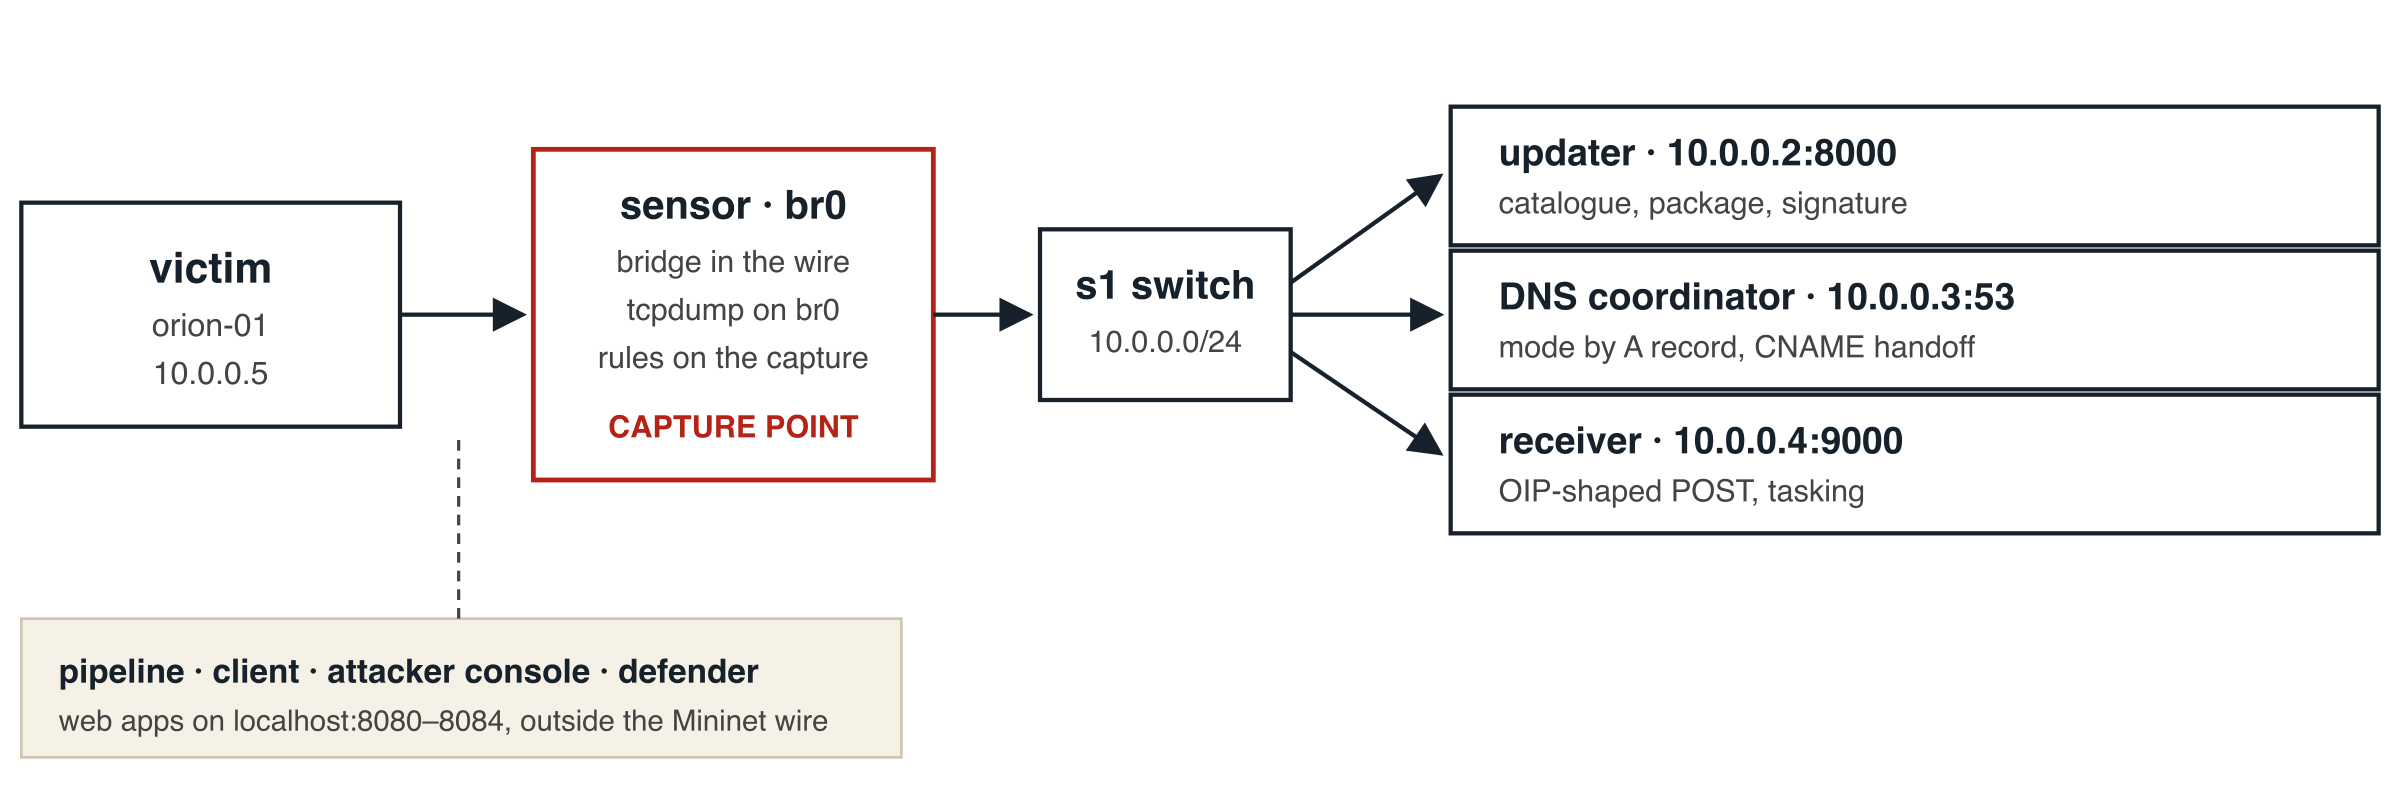
\includegraphics[width=\textwidth]{topology.png}
\caption{Lab topology. The victim reaches the switch only through the bridge, and the capture holds DNS, update and upload traffic on UDP/53, TCP/8000 and TCP/9000.}
\label{fig:topology}
\end{figure}

\subsection{Implemented chain}

Table~\ref{tab:killchain} maps the incident to the lab. The status column records what the demo runs: the release pipeline, the coordinator mode change, and a task from the operator console.

\begin{table}[H]
\centering
\footnotesize
\hyphenpenalty=10000
\caption{Kill-chain mapping. Implemented: the demo runs this step. Reduced: the trust failure is preserved, but not the actor's tooling or scale.}
\label{tab:killchain}
\begin{tabular}{@{}>{\RaggedRight}p{2.3cm}>{\RaggedRight}p{4.7cm}>{\RaggedRight}p{4.7cm}>{\RaggedRight}p{2.5cm}@{}}
\toprule
\textbf{Phase} & \textbf{In the incident} & \textbf{In the lab} & \textbf{Status} \\
\midrule
Reconnaissance & Build pipeline understood before SUNSPOT was written~\cite{crowdstrike-sunspot} & Nothing & Not modelled \\
Weaponization & Source file replaced during the build, original restored~\cite{crowdstrike-sunspot} & Higher public \texttt{orion-compat} replaces the component in the build workspace; the manifest is generated afterwards and records the component's hash & Performed, reduced \\
Delivery & Signed update through the normal channel~\cite{mandiant-campaign} & Signed package published to a stable channel, downloaded over HTTP & Implemented \\
Exploitation & No vulnerability; the customer trusts the signed package & No vulnerability; the client accepts V3 after all checks pass & Not applicable \\
Installation & Backdoored DLL loads inside Orion & Installer registers the component and starts one process per declaration (the manifest declares one) & Implemented, reduced \\
Command and control & DGA check-in, mode by A record, CNAME handoff, OIP-shaped HTTPS & Encoded check-in, mode by coordinator answer, CNAME used for resolution, HTTP to the bare IP & Implemented, reduced \\
Actions on objectives & TEARDROP to Cobalt Strike, AdFind, credential access, SAML forgery & A shell command and a decoy-file read, issued as PoC commands & Implemented, reduced \\
\bottomrule
\end{tabular}
\end{table}

The client accepts the malicious package because every check passes. The package digest matches the catalogue value, the signature verifies against the pinned key, and the component digest matches the SHA-256 the manifest declares. The package is still malicious.

After installation, the component waits three seconds, builds a base32 label from an XORed record holding a version byte, a mode byte, a user identifier, host and user names, and a CRC-16, and queries the coordinator. A bad checksum returns NXDOMAIN. The coordinator answers \texttt{192.0.2.10} for passive, \texttt{192.0.2.20} for selected (shown as ACTIVE), or NXDOMAIN when disabled. The component starts at mode 4, moves to 5 on the activation address, and exits after a final mode-3 check-in when the coordinator is disabled. The coordinator's CNAME is a fixed handoff name, not a DGA-generated record of the kind the real coordinator returned.

Active traffic goes to \texttt{/swip/upd/orion.improvementprogram.asmx} with an \texttt{Orion/2020.2.4} agent string and a body of fields modelled on the Improvement Program, including \texttt{customerId}, \texttt{machineName}, \texttt{userName}, \texttt{osVersion}, \texttt{ipAddress}, and \texttt{processId}. The receiver answers with \texttt{swip.tasks}, and the component returns output in a \texttt{telemetry} block. The demo sends PoC commands from the operator console.

\subsection{What the recreation does not do}

Weaponization is the largest gap. There is no Orion source build and no \texttt{MsBuild.exe} to watch, so SUNSPOT's replacement and restore is not reproduced. The lab's build trusts a public package that outranks the internal one and runs its install hook, which is dependency confusion rather than a source-file swap, and nothing restores an original. The pipeline copies an approved Python source tree and packages it. It does not compile an Orion product. The real incident used SUNSPOT to swap a source file; the lab models dependency confusion. The lab has no Windows host, no signed PE, and no DLL loaded inside a product. Dormancy is compressed from 12 to 14 days to three seconds, and the environment checks are omitted, which makes the lab implant more portable than the original. Check-ins repeat every four seconds against a real minimum of one minute for HTTP and sleeps measured in hours for DNS. The control channel is plain HTTP so the capture can be read, and the implant queries the coordinator directly instead of using the system resolver. It also posts to the address it resolved rather than to the CNAME host, so the lab exercises a bare-IP variant; the real implant used the hostname and required a preceding A record in specific ranges. There is one victim, no persistence, no second stage, and no lateral movement.

Table~\ref{tab:killchain} overstates completeness. The lab reproduces the trust path and the check-in sequence, not the actor's code.

\section{Detection}
\label{sec:detection}

The sensor reads the capture file the tap writes. Its rules inspect packets, not the DNS log, receiver log, or scenario state. A separate host sensor polls \texttt{/proc} every 250 ms, follows parent PIDs, and records start and stop events for the component and its descendants, including pid, user, role and command line. The Blue Team app lists those events beside the packet rules.

Table~\ref{tab:rules} lists the eight rules. Five run on the default demo; \texttt{T5-EXFIL-001} needs the optional collect task, and the self-test covers the lookalike and replay cases.

\begin{table}[H]
\centering
\footnotesize
\hyphenpenalty=10000
\caption{Sensor rules and the traffic each one inspects.}
\label{tab:rules}
\begin{tabular}{@{}>{\RaggedRight}p{2.2cm}>{\RaggedRight}p{6.4cm}>{\RaggedRight}p{2.7cm}>{\RaggedRight}p{2.8cm}@{}}
\toprule
\textbf{Rule} & \textbf{Signal} & \textbf{Source} & \textbf{Coverage} \\
\midrule
\texttt{T5-DGA-001} & Encoded label under the check-in suffix & DNS query & Demo \\
\texttt{T5-DGA-002} & Label decodes with a valid CRC-16 & DNS query & Demo \\
\texttt{T5-DGA-003} & Encoded shape, but invalid base32, version, length, or checksum & DNS query & Self-test \\
\texttt{T5-DGA-004} & Same decoded label from a second source address & DNS query & Self-test \\
\texttt{T5-BCN-001} & Stable interval across successive check-ins & DNS timing & Demo \\
\texttt{T5-C2-001} & First contact with a new destination & Any flow & Demo \\
\texttt{T5-C2-002} & Improvement Program POST to a non-global address, or an \texttt{Orion/} agent & HTTP & Demo \\
\texttt{T5-EXFIL-001} & POST above 4 KB to a non-global address & HTTP & Optional collect \\
\bottomrule
\end{tabular}
\end{table}

The check-in label decodes to a host name, user, uid, mode byte, and CRC-16. The interval between queries stays close to four seconds, and each active check-in produces an Improvement Program POST. Once captured, the check-in is decodable and periodic, and the telemetry upload is visible on the wire.

The sensor also records CNAME responses. Mandiant treats a CNAME resolution as a stronger signal than a decoded label, because a decoded label shows that the implant ran while a CNAME can point to follow-on control~\cite{mandiant-sunburst-details}.

\section{Countermeasures}
\label{sec:countermeasures}

Before signing, the controls address the build itself. Separating build infrastructure from office networks, restricting outbound traffic, using short-lived agents, and limiting who can change build jobs all reduce the opportunity SUNSPOT used. CISA recommends restricting access to code and build systems and separating build infrastructure from other networks (p.~12)~\cite{cisa-supply-chain}. Comparing a released artefact with an independently produced reference, or rebuilding from source and comparing hashes, targets the substitution directly. Neither proves the code is benign; a reproducible malicious build is still malicious.

At the customer, least privilege and restricted update permissions limit what an installed component can do. A traffic baseline is a detection control and belongs with the network monitoring below, not with prevention. SBOMs and supplier assessments shorten the time to identify affected components but do not prevent the build compromise (pp.~7 and 13)~\cite{cisa-supply-chain}.

After installation, detection depends on behaviour. DNS logging and anomaly analysis can show an unexpected check-in, and network baselines can separate vendor telemetry from a lookalike. EDR has little to work with while a signed component behaves normally, but becomes useful when the operator acts. CISA's Orion guidance covers reviewing stored traffic for new external DNS domains and comparing a product's expected external communications with what is observed~\cite{cisa-aa20-352a,cisa-supply-chain}.

Table~\ref{tab:countermeasures} rates each control for expected effectiveness and deployment difficulty. The ratings are this article's judgement on a four-point scale (low, medium, high, very high), not measurements from the lab.

\begin{table}[H]
\centering
\footnotesize
\hyphenpenalty=10000
\caption{Countermeasures by stage, with expected effectiveness and deployment difficulty.}
\label{tab:countermeasures}
\begin{tabular}{@{}>{\RaggedRight}p{3.5cm}>{\RaggedRight}p{2.4cm}>{\RaggedRight}p{2.1cm}>{\RaggedRight}p{6.6cm}@{}}
\toprule
\textbf{Countermeasure} & \textbf{Effectiveness} & \textbf{Difficulty} & \textbf{Reason} \\
\midrule
Build pipeline isolation & High & High & Rebuilds infrastructure, network controls, and developer workflow \\
Reproducible builds & High & Very high & Catches tampering, but needs pinned dependencies, deterministic toolchains, and controlled timestamps \\
Independent artefact verification & High & High & Needs a separate verification path, trusted records, and a release gate \\
HSM-protected signing keys & Low & Medium & Protects the signing step, which the attackers did not need to break \\
DNS anomaly detection & Medium & Medium & Gives visibility, but needs logging and tuning; a fixed-domain lab is not a DGA test \\
Network behaviour analysis & Medium & High & Needs a baseline before deviations mean anything \\
EDR & Medium & Medium & Limited against a signed passive component \\
MFA and least privilege & Medium & Low & Limits movement, not the initial update \\
SBOM and vendor risk management & Low & Medium & Gives visibility rather than prevention \\
\bottomrule
\end{tabular}
\end{table}

The controls with the most effect are also the hardest to deploy, which is the practical problem with supply-chain defence. A customer cannot verify a build it did not perform, and a supplier cannot prove a build was clean without records the attacker could not alter.

\section{Academic literature}
\label{sec:literature}

Six peer-reviewed papers bear on the stages the lab implements. The selection rule was publication between 2019 and 2026 in a peer-reviewed venue, with a direct bearing on build integrity, release verification, or network detection of the command channel. Three come from flagship venues (USENIX Security, IEEE S\&P, ICSE); the others are DIMVA and two journals. Studies of open-source package ecosystems are treated as analogous evidence, not as analyses of Orion.

in-toto (USENIX Security 2019) checks that authorised actors performed the expected steps in a supply chain and that materials and products match recorded evidence. The authors mapped it retrospectively to 30 historical compromises. It addresses the gap SUNSPOT exploited, with the caveat that it depends on trusted policy, keys, and redundant builds~\cite{intoto}.

The Backstabber's Knife Collection (DIMVA 2020) analysed 469 malicious packages in npm, PyPI, and RubyGems, and studied 174 of them. Trusted distribution can carry malicious code, and conditional execution makes it hard to observe. The sample is open source, so it supports the trust failure but not the build compromise~\cite{backstabber}.

The SoK taxonomy by Ladisa et al.\ (IEEE S\&P 2023) separates build-time compromise from distribution and maps 107 attack vectors to safeguards. It places the lab's scenario and the controls in Section~\ref{sec:countermeasures}, but its mappings are not test results~\cite{sok-taxonomy}.

Gokkaya et al.\ (JISA 2026) reviews the supply-chain literature and argues for prioritising controls by risk rather than applying all of them. It frames the mitigation discussion and does not evaluate SolarWinds defences~\cite{gokkaya}.

Benedetti et al.\ (ICSE 2025) sampled six package ecosystems; Go ships no artefacts, so five produce reproducibility rates. We take from this that a signature says nothing about the build behind it, and that an independent rebuild gives a comparison point. The paper does not perform that comparison, and reproducibility does not prove benign code~\cite{reproducible}.

Manasrah et al.\ (JKSU-CIS 2022) detected DGA domains from lexical features of query names. SUNBURST used DNS for control, so query-name telemetry is worth monitoring. The study analyses registrable domains, not subdomains or CNAME targets, so it supports check-in monitoring but not the handoff the lab demonstrates~\cite{dga-detection}.

\begin{table}[H]
\centering
\footnotesize
\caption{The reviewed papers, their evidence, and what each supports in this article.}
\label{tab:papers}
\begin{tabular}{@{}>{\RaggedRight}p{2.3cm}>{\RaggedRight}p{3.3cm}>{\RaggedRight}p{4.2cm}>{\RaggedRight}p{4.9cm}@{}}
\toprule
\textbf{Paper} & \textbf{Evidence} & \textbf{Stage} & \textbf{Limit for this study} \\
\midrule
in-toto (2019) & Framework and retrospective mapping & Build and release & Needs trusted policy, keys, and redundant builds \\
Backstabber's Knife (2020) & Manual package study & Dependency and execution & Open-source sample, not Orion \\
Ladisa et al.\ (2023) & Taxonomy and expert surveys & Entire supply chain & Mappings are not PoC results \\
Gokkaya et al.\ (2026) & Systematic review & Risk management & No SolarWinds-specific experiment \\
Benedetti et al.\ (2025) & Multi-ecosystem measurement & Build and artifact integrity & Reproducibility does not prove benign code \\
Manasrah et al.\ (2022) & DNS query-name classification & Post-installation network & No subdomain or CNAME analysis \\
\bottomrule
\end{tabular}
\end{table}

Provenance checks address the build, and DNS monitoring addresses behaviour after installation. A signature addresses neither, and none of the six papers tests the pair together on a signed-update workflow.

\section{Research question}
\label{sec:question}

None of the six papers reviewed here tests provenance verification, independent rebuilding, and DNS monitoring together. The proof-of-concept (PoC) uses DNS monitoring for detection only; the resolver block is an operator action, not a monitoring-driven defence. It compares an unsigned catalogue digest and verifies the package signature, but it implements no independent verification: no rebuild and no reference-artefact comparison. The article therefore asks:

\begin{quote}
\textbf{Which stages of a compromised but legitimately signed software-update workflow can independent build-artefact verification and DNS activity monitoring identify in a controlled Mininet and Docker lab, and how many false positives does each control produce?}
\end{quote}

Three sub-questions separate the stages. Before release, can an independently generated reference artefact or a trusted provenance policy distinguish the malicious V3 from an approved release when both pass signature checks? After installation, which check-ins and CNAME handoffs does DNS logging reveal, and how many alerts does a stated rule raise on benign runs? And which stages remain invisible when either control is used alone?

The evaluation would run a baseline approved update, the tampered update, an artefact comparison, DNS monitoring on labelled runs, and both controls together. It would record detected releases, flagged check-ins, false positives on benign runs, and the stage at which each alert fires. The lab has no benign DNS workload at present, so the false-positive half of the question is not yet measurable; benign comparison traffic is required before any detection rate means anything. If reproducible builds cannot be implemented, an approved-reference comparison is the narrower fallback, and it must not be described as proof of reproducible-build security.

The limits are the lab's: a predefined check-in routine, simplified DNS, no SUNSPOT replacement, no original DGA, and no later-stage malware. Results would describe this environment, not SolarWinds.

\section{Conclusion}
\label{sec:conclusion}

The SolarWinds campaign worked because the attackers did not need to break a defence. They used the supplier's build and signing process, and customers installed the result with every check passing. The lab reproduces that trust failure and the check-in sequence that followed, and it stops where the intrusion began: no second stage, no lateral movement, no collection.

A signature identifies the signer. Build isolation, provenance records, and independent verification act before the signature exists, while DNS and network monitoring act after installation. The papers support both layers, and none tests them together in a lab like this one, which is what the research question proposes to do.


\phantomsection
\addcontentsline{toc}{section}{References}
\begin{thebibliography}{99}
\small
\raggedright
\setlength{\itemsep}{1pt}

\bibitem{mitre-apt29} MITRE ATT\&CK. ``APT29.'' Group G0016. \url{https://attack.mitre.org/groups/G0016/}

\bibitem{aa22-110a} U.S., Australian, Canadian, New Zealand, and UK cybersecurity authorities. ``Russian State-Sponsored and Criminal Cyber Threats to Critical Infrastructure.'' Joint Cybersecurity Advisory AA22-110A, 20 April 2022. \url{https://www.cisa.gov/news-events/cybersecurity-advisories/aa22-110a}

\bibitem{eset-ghost} ESET. ``Operation Ghost Hunt: The DNC hacking group `Dukes' still attacks government targets, ESET discovers.'' 17 October 2019. \url{https://www.eset.com/us/about/newsroom/press-releases/operation-ghost-hunt-the-dnc-hacking-group-dukes-still-attacks-government-targets-eset-discovers-1/}

\bibitem{crowdstrike-dnc} Dmitri Alperovitch, CrowdStrike. ``Bears in the Midst: Intrusion Into the Democratic National Committee.'' 14 June 2016; reproduced in CrowdStrike's 4 June 2020 retrospective. \url{https://www.crowdstrike.com/en-us/blog/bears-midst-intrusion-democratic-national-committee/}

\bibitem{ncsc-vaccine} UK NCSC and Communications Security Establishment Canada. ``Advisory: APT29 targets COVID-19 vaccine development.'' 16 July 2020. \url{https://www.ncsc.gov.uk/news/advisory-apt29-targets-covid-19-vaccine-development}

\bibitem{mandiant-campaign} FireEye/Mandiant. ``Highly Evasive Attacker Leverages SolarWinds Supply Chain to Compromise Multiple Global Victims With SUNBURST Backdoor.'' 13 December 2020. \url{https://cloud.google.com/blog/topics/threat-intelligence/evasive-attacker-leverages-solarwinds-supply-chain-compromises-with-sunburst-backdoor}

\bibitem{mandiant-sunburst-details} Stephen Eckels, Jay Smith, and William Ballenthin, Mandiant. ``SUNBURST Additional Technical Details.'' 24 December 2020. \url{https://cloud.google.com/blog/topics/threat-intelligence/sunburst-additional-technical-details}

\bibitem{crowdstrike-sunspot} CrowdStrike Intelligence Team. ``SUNSPOT: An Implant in the Build Process.'' 11 January 2021. \url{https://www.crowdstrike.com/en-us/blog/sunspot-malware-technical-analysis/}

\bibitem{microsoft-teardrop} Microsoft. ``Deep dive into the Solorigate second-stage activation: From SUNBURST to TEARDROP and Raindrop.'' 20 January 2021. \url{https://www.microsoft.com/en-us/security/blog/2021/01/20/deep-dive-into-the-solorigate-second-stage-activation-from-sunburst-to-teardrop-and-raindrop/}

\bibitem{solarwinds-sec} SolarWinds. ``An Investigative Update of the Cyberattack.'' Form 8-K exhibit, 7 May 2021. \url{https://www.sec.gov/Archives/edgar/data/1739942/000173994221000076/swi-20210507.htm}

\bibitem{gao} U.S. Government Accountability Office. ``Cybersecurity: Federal Response to SolarWinds and Microsoft Exchange Incidents.'' GAO-22-104746, 13 January 2022, pp.~16--17. \url{https://www.gao.gov/products/gao-22-104746}

\bibitem{task05lab} Task 5 lab. \texttt{tasks/task05-poc}, commit \texttt{7c99000}, 25 November 2026. \url{https://github.com/Sirbu-Boeti-Eduard/cdci_apt29_study}

\bibitem{cisa-aa20-352a} CISA. ``Advanced Persistent Threat Compromise of Government Agencies, Critical Infrastructure, and Private Sector Organizations.'' AA20-352A, 17 December 2020, updated 15 April 2021. \url{https://www.cisa.gov/news-events/cybersecurity-advisories/aa20-352a}

\bibitem{sec-mimecast} U.S. Securities and Exchange Commission. ``In the Matter of Mimecast Limited.'' Release 33-11322, 22 October 2024. \url{https://www.sec.gov/files/litigation/admin/2024/33-11322.pdf}

\bibitem{mimecast-10k} Mimecast. FY2021 Form 10-K. Filed 27 May 2021. \url{https://www.sec.gov/Archives/edgar/data/1644675/000156459021030433/mime-10k_20210331.htm}

\bibitem{doj-statement} U.S. Department of Justice, Office of Privacy and Civil Liberties. ``Department of Justice Statement on the intrusion into the Department's Microsoft O365 email environment.'' Updated 12 October 2022. \url{https://www.justice.gov/opcl/department-justice-statement-intrusion-department-s-microsoft-o365-email-environment}

\bibitem{doj-review} U.S. Department of Justice. ``Comprehensive Cyber Review.'' 1 July 2022. \url{https://www.justice.gov/usdoj-media/dag/media/1232936/dl?inline=}

\bibitem{sec-checkpoint} U.S. Securities and Exchange Commission. ``In the Matter of Check Point Software Technologies Ltd.'' Release 33-11321, 22 October 2024. \url{https://www.sec.gov/files/litigation/admin/2024/33-11321.pdf}

\bibitem{fireeye-hammertoss} FireEye Threat Intelligence. ``HAMMERTOSS: Stealthy Tactics Define a Russian Cyber Threat Group.'' July 2015. \url{https://services.google.com/fh/files/misc/rpt-apt29-hammertoss-stealthy-tactics-define-en.pdf}

\bibitem{aa21-116a} CISA, FBI, and DHS. ``Russian Foreign Intelligence Service (SVR) Cyber Operations: Trends and Best Practices for Network Defenders.'' AA21-116A, 26 April 2021. \url{https://www.cisa.gov/news-events/cybersecurity-advisories/aa21-116a}

\bibitem{ms-nobelium} Tom Burt, Microsoft. ``Another Nobelium cyberattack.'' 27 May 2021. \url{https://blogs.microsoft.com/on-the-issues/2021/05/27/nobelium-cyberattack-nativezone-solarwinds/}

\bibitem{skw-certpolska} Military Counterintelligence Service (SKW) and CERT Polska. ``Espionage campaign linked to Russian intelligence services.'' 13 April 2023. \url{https://www.gov.pl/web/baza-wiedzy/espionage-campaign-linked-to-russian-intelligence-services}

\bibitem{unit42} Unit 42, Palo Alto Networks. ``Diplomats Beware: Cloaked Ursa Phishing With a Twist.'' 12 July 2023, updated 20 July 2023. \url{https://unit42.paloaltonetworks.com/cloaked-ursa-phishing/}

\bibitem{ms-teams} Microsoft Threat Intelligence. ``Midnight Blizzard conducts targeted social engineering over Microsoft Teams.'' 2 August 2023. \url{https://www.microsoft.com/en-us/security/blog/2023/08/02/midnight-blizzard-conducts-targeted-social-engineering-over-microsoft-teams/}

\bibitem{mandiant-wineloader} Luke Jenkins and Dan Black, Mandiant. ``APT29 Uses WINELOADER to Target German Political Parties.'' 22 March 2024. \url{https://cloud.google.com/blog/topics/threat-intelligence/apt29-wineloader-german-political-parties}

\bibitem{ms-rdp} Microsoft Threat Intelligence. ``Midnight Blizzard conducts large-scale spear-phishing campaign using RDP files.'' 29 October 2024. \url{https://www.microsoft.com/en-us/security/blog/2024/10/29/midnight-blizzard-conducts-large-scale-spear-phishing-campaign-using-rdp-files/}

\bibitem{checkpoint-2025} Check Point Research. ``Renewed APT29 Phishing Campaign Against European Diplomats.'' 15 April 2025. \url{https://research.checkpoint.com/2025/apt29-phishing-campaign/}

\bibitem{cisa-supply-chain} CISA. ``Defending Against Software Supply Chain Attacks.'' April 2021. \url{https://www.cisa.gov/sites/default/files/publications/defending_against_software_supply_chain_attacks_508_1.pdf}

\bibitem{intoto} S. Torres-Arias, H. Afzali, T. K. Kuppusamy, R. Curtmola, and J. Cappos. ``in-toto: Providing farm-to-table guarantees for bits and bytes.'' 28th USENIX Security Symposium, pp.~1393--1410, 2019. \url{https://www.usenix.org/conference/usenixsecurity19/presentation/torres-arias}

\bibitem{backstabber} M. Ohm, H. Plate, A. Sykosch, and M. Meier. ``Backstabber's Knife Collection: A Review of Open Source Software Supply Chain Attacks.'' DIMVA 2020, LNCS 12223, pp.~23--43. \url{https://doi.org/10.1007/978-3-030-52683-2_2}

\bibitem{sok-taxonomy} P. Ladisa, H. Plate, M. Martinez, and O. Barais. ``SoK: Taxonomy of Attacks on Open-Source Software Supply Chains.'' 2023 IEEE Symposium on Security and Privacy, pp.~1509--1526. \url{https://doi.org/10.1109/SP46215.2023.10179304}

\bibitem{gokkaya} B. Gokkaya, L. Aniello, and B. Halak. ``Software supply chain: A taxonomy of attacks, mitigations and risk assessment strategies.'' Journal of Information Security and Applications, vol.~97, art.~104324, 2026. \url{https://doi.org/10.1016/j.jisa.2025.104324}

\bibitem{reproducible} G. Benedetti et al. ``An Empirical Study on Reproducible Packaging in Open-Source Ecosystems.'' ICSE 2025, pp.~1052--1063. \url{https://doi.org/10.1109/ICSE55347.2025.00136}

\bibitem{dga-detection} A. M. Manasrah, T. Khdour, and R. Freehat. ``DGA-based botnets detection using DNS traffic mining.'' Journal of King Saud University -- Computer and Information Sciences, vol.~34, no.~5, pp.~2045--2061, 2022. \url{https://doi.org/10.1016/j.jksuci.2022.03.001}

\bibitem{mandiant-unc2452} Mandiant. ``Assembling the Russian Nesting Doll: UNC2452 Merged into APT29.'' 27 April 2022. \url{https://cloud.google.com/blog/topics/threat-intelligence/unc2452-merged-into-apt29}

\bibitem{aa23-347a} CISA, FBI, NSA, SKW, CERT Polska, and NCSC. ``Russian Foreign Intelligence Service (SVR) Exploiting JetBrains TeamCity CVE Globally.'' AA23-347A, 13 December 2023. \url{https://www.cisa.gov/news-events/cybersecurity-advisories/aa23-347a}

\bibitem{nsa-svr} NSA, CISA, and FBI. ``Russian SVR Targets U.S. and Allied Networks.'' 15 April 2021. \url{https://media.defense.gov/2021/apr/15/2002621240/-1/-1/0/csa_svr_targets_us_allies_uoo13234021.pdf}

\end{thebibliography}

\vspace{6pt}
\noindent\footnotesize All URLs were retrieved on 25 November 2026.


\end{document}
